\documentclass[12pt]{article}
\usepackage[utf8]{inputenc}
\usepackage{geometry}
\geometry{a4paper, margin=1in}
\usepackage{amsmath}
\usepackage{amsfonts}
\usepackage{graphicx}
\usepackage{hyperref}
\usepackage{booktabs}
\usepackage{xcolor}
\usepackage{listings}

\hypersetup{
    colorlinks=true,
    linkcolor=blue,
    filecolor=magenta,
    urlcolor=blue,
}

\title{ME 759 Final Project Report\\ \Large FlashAttention in Raw CUDA}
\author{Gaurav Batra \\ \href{mailto:gbatra3@wisc.edu}{gbatra3@wisc.edu} \\ \textit{Computer Science (MS)}}
\date{May 3, 2026}

\begin{document}

\maketitle

\vspace{-1.5em}
\begin{center}
    \textbf{Project Repository:} \url{https://github.com/batra98/me759-flashattention} \\
    \vspace{0.3em}
    \textbf{Interactive Educational Report:} \url{https://batra98.github.io/me759-flashattention}
\end{center}
\vspace{1em}

\begin{abstract}
Standard Transformer attention mechanisms suffer from $O(N^2)$ memory complexity. Calculating the dot product of every Query with every Key requires materializing a massive $N \times N$ matrix in High Bandwidth Memory (HBM). This report describes a custom FlashAttention forward pass in bare-metal CUDA. By utilizing Shared Memory (SRAM) and reformulating the softmax computation, we demonstrate a reduction in global memory traffic from $O(N^2)$ to $O(N)$; on an NVIDIA Tesla T4 at $N{=}4096$, FlashAttention v1 (FP32 tiling) achieves roughly a $1.8\times$ speedup over a three-kernel naive baseline and orders-of-magnitude lower HBM writes versus materializing $S$. We additionally evaluate causal masking, a warp-shuffle row formulation, and a WMMA Tensor Core score path behind the same \texttt{flash\_attn} driver: at $N{=}8192$, causal FlashAttention reaches $\approx 30.6$\,ms vs.\ $\approx 58.7$\,ms for non-causal Flash and $\approx 112$\,ms for naive; WMMA improves non-causal Flash to $\approx 50.0$\,ms while NCU global-byte counters remain lowest for WMMA. An interactive educational website visualizes the Streaming Multiprocessor (SM) memory hierarchy.
\end{abstract}

\section{Introduction and Motivation}
In modern Deep Learning workloads, specifically autoregressive large language models, inference is fundamentally memory-bandwidth bound rather than compute-bound \cite{dao2022}. The standard attention formulation materializes the full $N \times N$ attention matrix $S$ in Global Memory (HBM). For sequence lengths like $N=4096$, writing this intermediate matrix to global memory, only to immediately read it back to compute the Softmax denominator, completely saturates the GPU memory bus.

While libraries like cuBLAS are highly optimized, they act as black boxes. Writing a custom FlashAttention kernel from scratch provides a deep understanding of hardware utilization. The objective of this project is to implement FlashAttention \cite{dao2022} completely from scratch in raw CUDA C++, benchmarking its latency and using NVIDIA Nsight Compute (NCU) to analytically verify the reduction in HBM traffic on an NVIDIA GPU.

\section{Methodology \& Algorithm Design}

\subsection{The Baseline (Naive) Implementation}
To form a solid experimental baseline, a standard three-kernel attention mechanism was implemented:
\begin{enumerate}
    \item \textbf{Score Kernel:} Computes $S = QK^T / \sqrt{d}$ and saves the full $N \times N$ matrix to HBM.
    \item \textbf{Softmax Kernel:} Loads rows from HBM, finds the moving maximum, exponentiates, and normalizes in a multi-pass approach over HBM lines.
    \item \textbf{Output Kernel:} Loads probabilities and $V$ from HBM, computing and writing the final output $O$ to HBM.
\end{enumerate}
This naive approach exhibits massive uncoalesced global reads and creates immense HBM thrashing.

For causal (autoregressive) comparisons we also implement \textbf{naive causal} attention: disallowed logits are set to large negative values before softmax, matching lower-triangular masking.

\subsection{FlashAttention (Tiled, Shared Memory) Implementation}
To resolve the memory bottleneck, the algorithm was redesigned to leverage the 64 KB Shared memory (SRAM) available per SM on the Tesla T4 architecture. With chosen block sizes $B_r = 32$, $B_c = 32$, and $d = 64$, the required matrices fit comfortably into a 24 KB SRAM footprint.

\subsubsection{Online Softmax and Loop Tiling}
Instead of processing the entire $N \times N$ matrix at once, the $Q, K,$ and $V$ matrices are sliced into smaller blocks. We load a small block from global memory into SRAM and compute the attention scores.

To prevent numerical overflow without requiring the entire row, we implement the Online Softmax algorithm \cite{milakov2018}. By maintaining a moving maximum ($m$) and a local normalization sum ($\ell$) directly within the ultra-fast thread registers, the denominator is updated incrementally:
\begin{equation}
m^{(j)}_i = \max\!\bigl(m^{(j-1)}_i,\; \tilde{m}_{ij}\bigr)
\end{equation}
\begin{equation}
\ell^{(j)}_i = e^{m^{(j-1)}_i - m^{(j)}_i}\,\ell^{(j-1)}_i + e^{\tilde{m}_{ij} - m^{(j)}_i}\,\tilde{\ell}_{ij}
\end{equation}
This allows the kernel to fuse the operations. The $O(N^2)$ logits are never written to HBM, as shown in this core CUDA block:

\begin{lstlisting}[language=C++, basicstyle=\ttfamily\footnotesize, frame=single, commentstyle=\color{green!60!black}]
// Online rescale: completely eliminating global memory writes
float m_new = fmaxf(m_i, m_tilde);
float alpha = expf(m_i - m_new);
float beta  = expf(m_tilde - m_new);

for (int k = 0; k < d; ++k) {
    float pv_k = 0.0f;
    for (int jj = 0; jj < bc_actual; ++jj)
        pv_k += S_row[jj] * V_smem[jj][k];
    O_acc[k] = alpha * O_acc[k] + beta * pv_k;
}
m_i = m_new;
l_i = alpha * l_i + beta * l_tilde;
\end{lstlisting}

\subsection{Causal FlashAttention}
For autoregressive masking we add \texttt{flash\_attention\_v1\_causal}: column tiles of $K/V$ that lie entirely in the future for the current $Q$ tile are skipped; within partially valid tiles, logits with $j>i$ are masked before the tile-wise softmax statistics.

\subsection{Warp-Shuffle Row Kernel (\texttt{flash\_v2})}
\texttt{flash\_attention\_v2.cu} assigns one warp per query row ($B_r{=}8$, $B_c{=}32$, $256$ threads per block). Dot products use warp reductions (\texttt{\_\_shfl\_down\_sync}); Section~\ref{sec:discussion} summarizes measured performance.

\subsection{WMMA Tensor Core Kernel (\texttt{flash\_wmma})}
\texttt{flash\_attention\_v3\_wmma.cu} computes $16{\times}16$ score tiles with WMMA \texttt{m16n16k16} on FP16 operands in shared memory while keeping softmax state in FP32. \texttt{flash\_wmma\_db} uses the same kernel body on sm\_75 as a control for double-buffering claims without an Ampere-style async copy path.

\section{Experimental Setup}
\begin{itemize}
    \item \textbf{Hardware:} NVIDIA Tesla T4 (sm\_75, Turing Architecture, 8.1 TFLOPs FP32).
    \item \textbf{Compilation:} Compiled using \texttt{nvcc} via CMake with \texttt{-O3 --extended-lambda --expt-relaxed-constexpr -lineinfo}.
    \item \textbf{Validation:} Root Mean Square Error (RMSE) against naive references; WMMA targets use a slightly looser FP16 tolerance where noted in code.
    \item \textbf{Measurement Tooling:} \texttt{cudaEvent} for latency, and \texttt{ncu} (NVIDIA Nsight Compute) for L1TEX bytes traffic evaluation.
\end{itemize}

\section{Results \& Benchmarks}

\subsection{Execution Latency (Speedup)}
FlashAttention exhibits steady and significant speedups over the naive baseline. At $N{=}4096$, latency improves from $\approx 27.03$\,ms to $\approx 15.05$\,ms ($\approx 1.8\times$). At $N{=}8192$, naive $\approx 111.99$\,ms vs.\ Flash v1 $\approx 58.68$\,ms.

\begin{figure}[htbp]
    \centering
    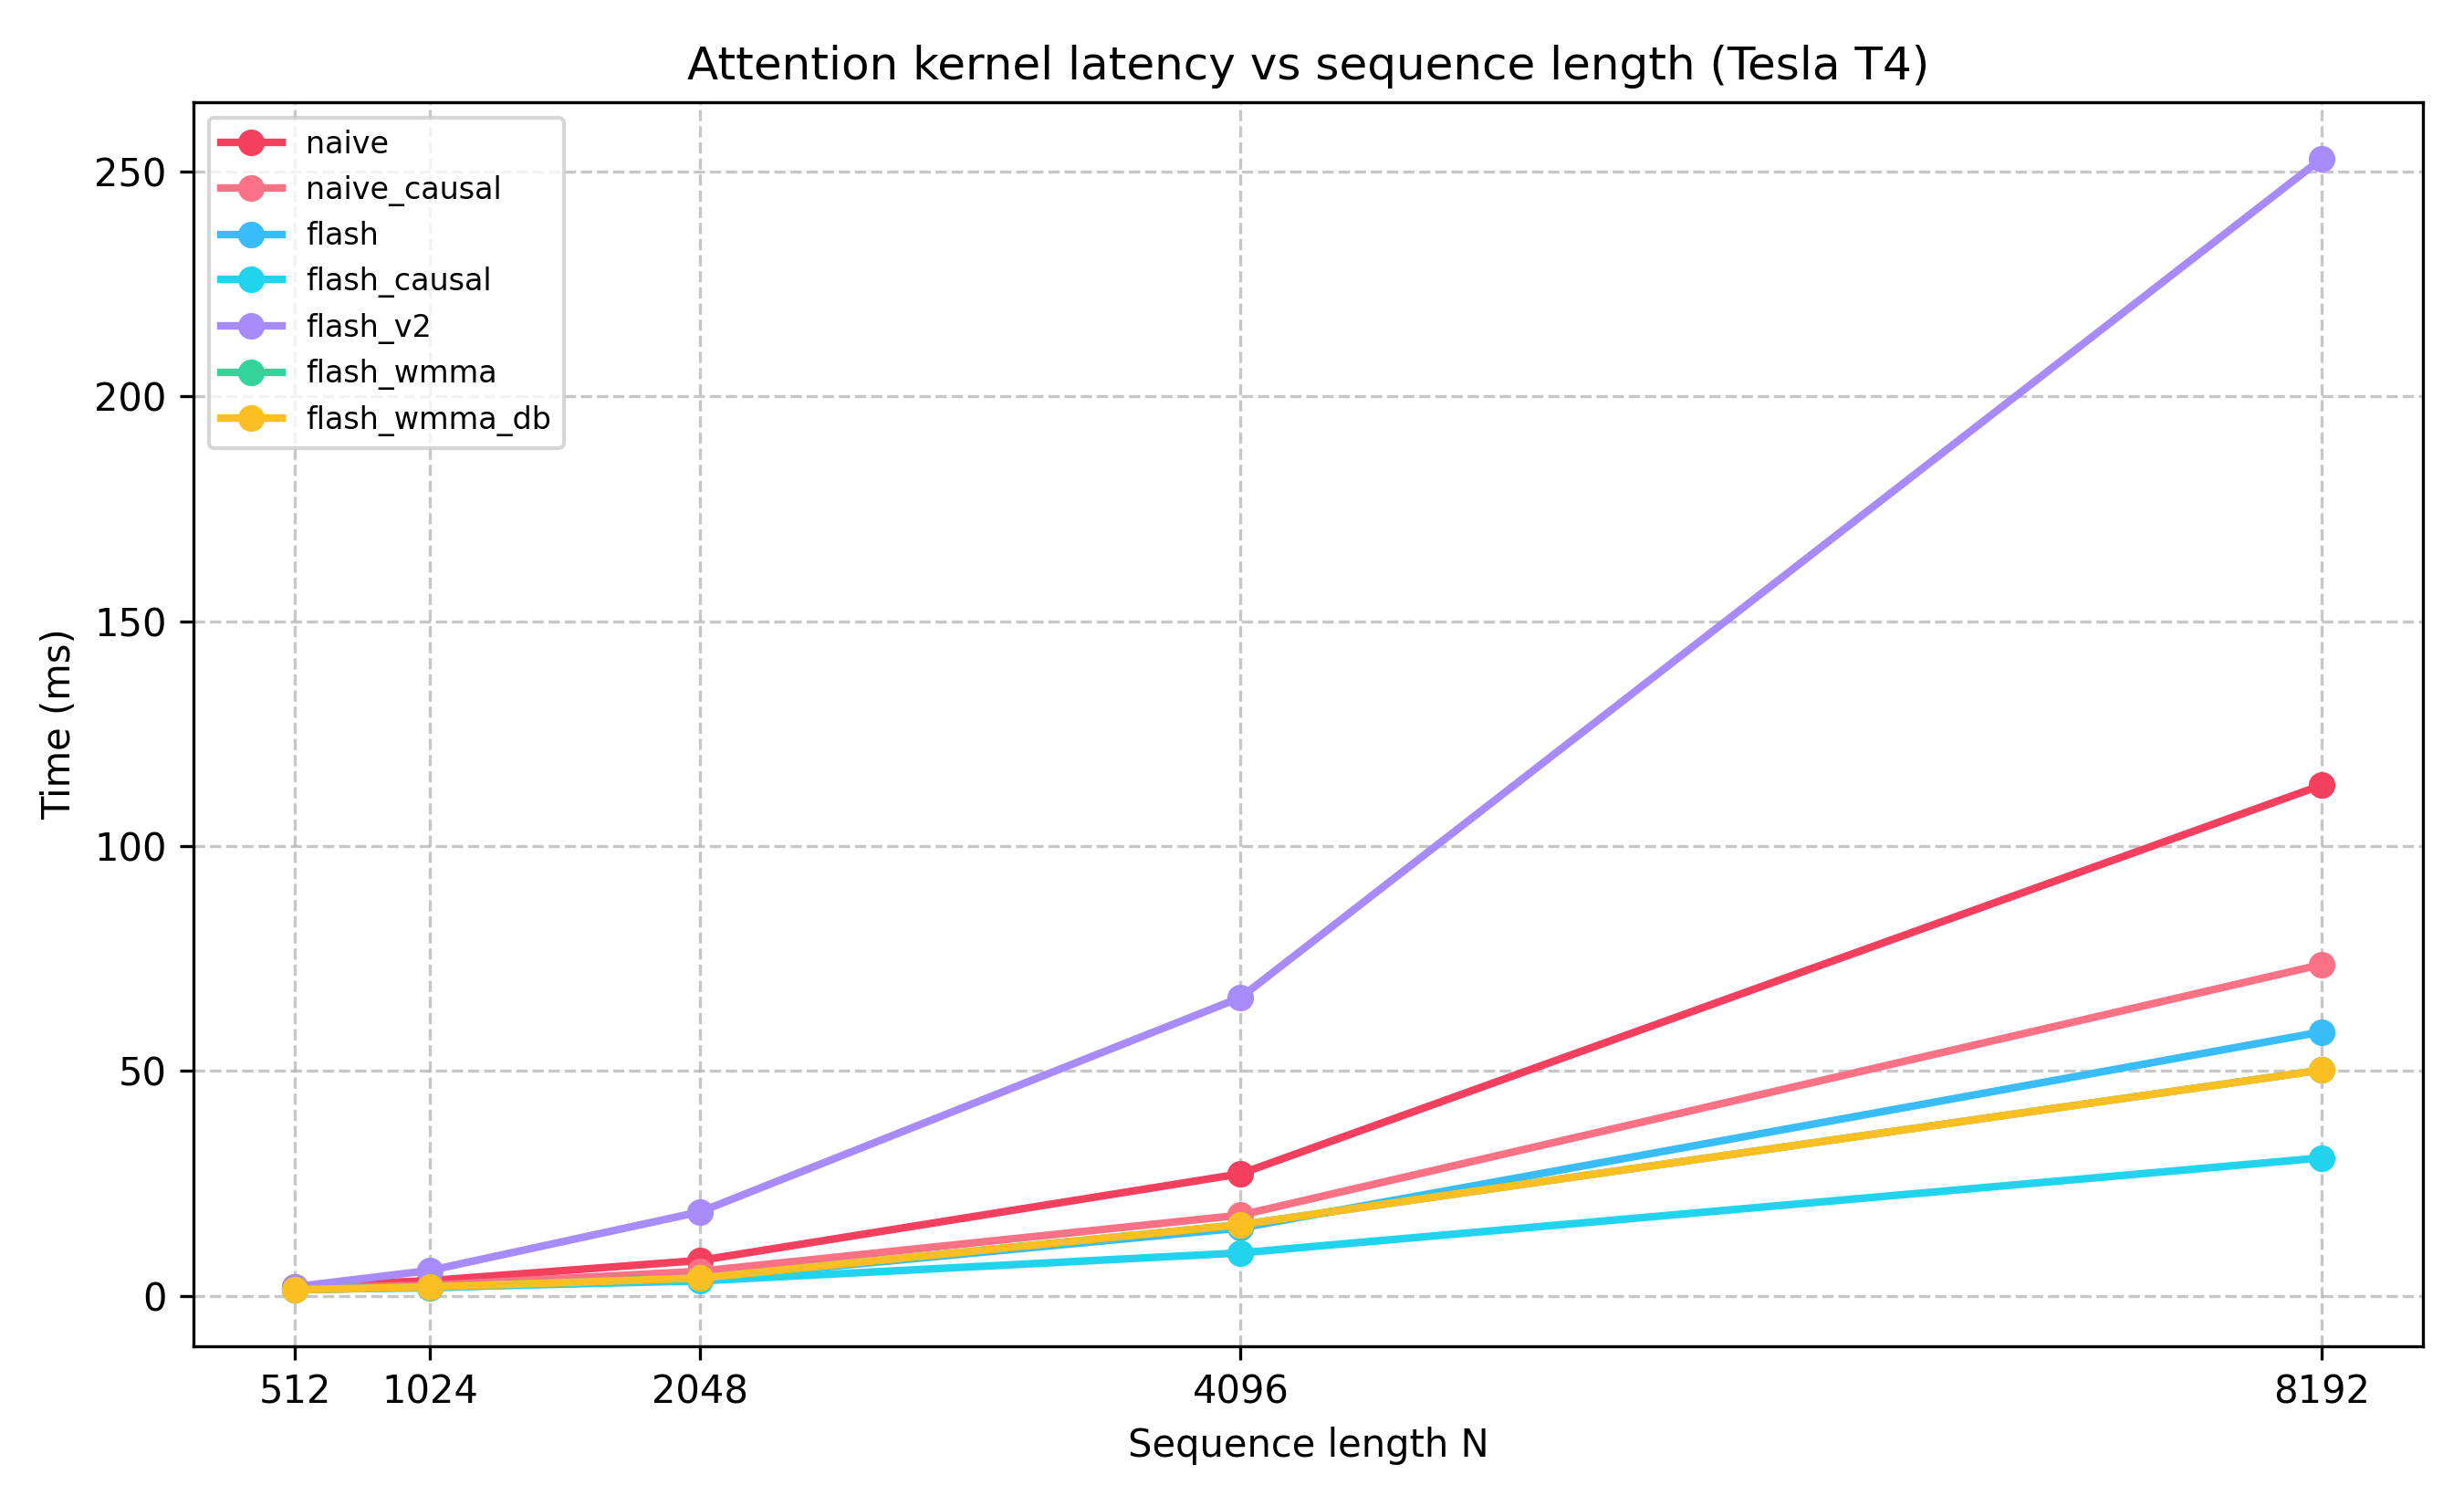
\includegraphics[width=0.75\textwidth]{docs/assets/latency_plot.png}
    \caption{Execution latency vs.\ sequence length (all kernels in \texttt{benchmarks/results/timing.csv}).}
    \label{fig:latency}
\end{figure}

\begin{figure}[htbp]
    \centering
    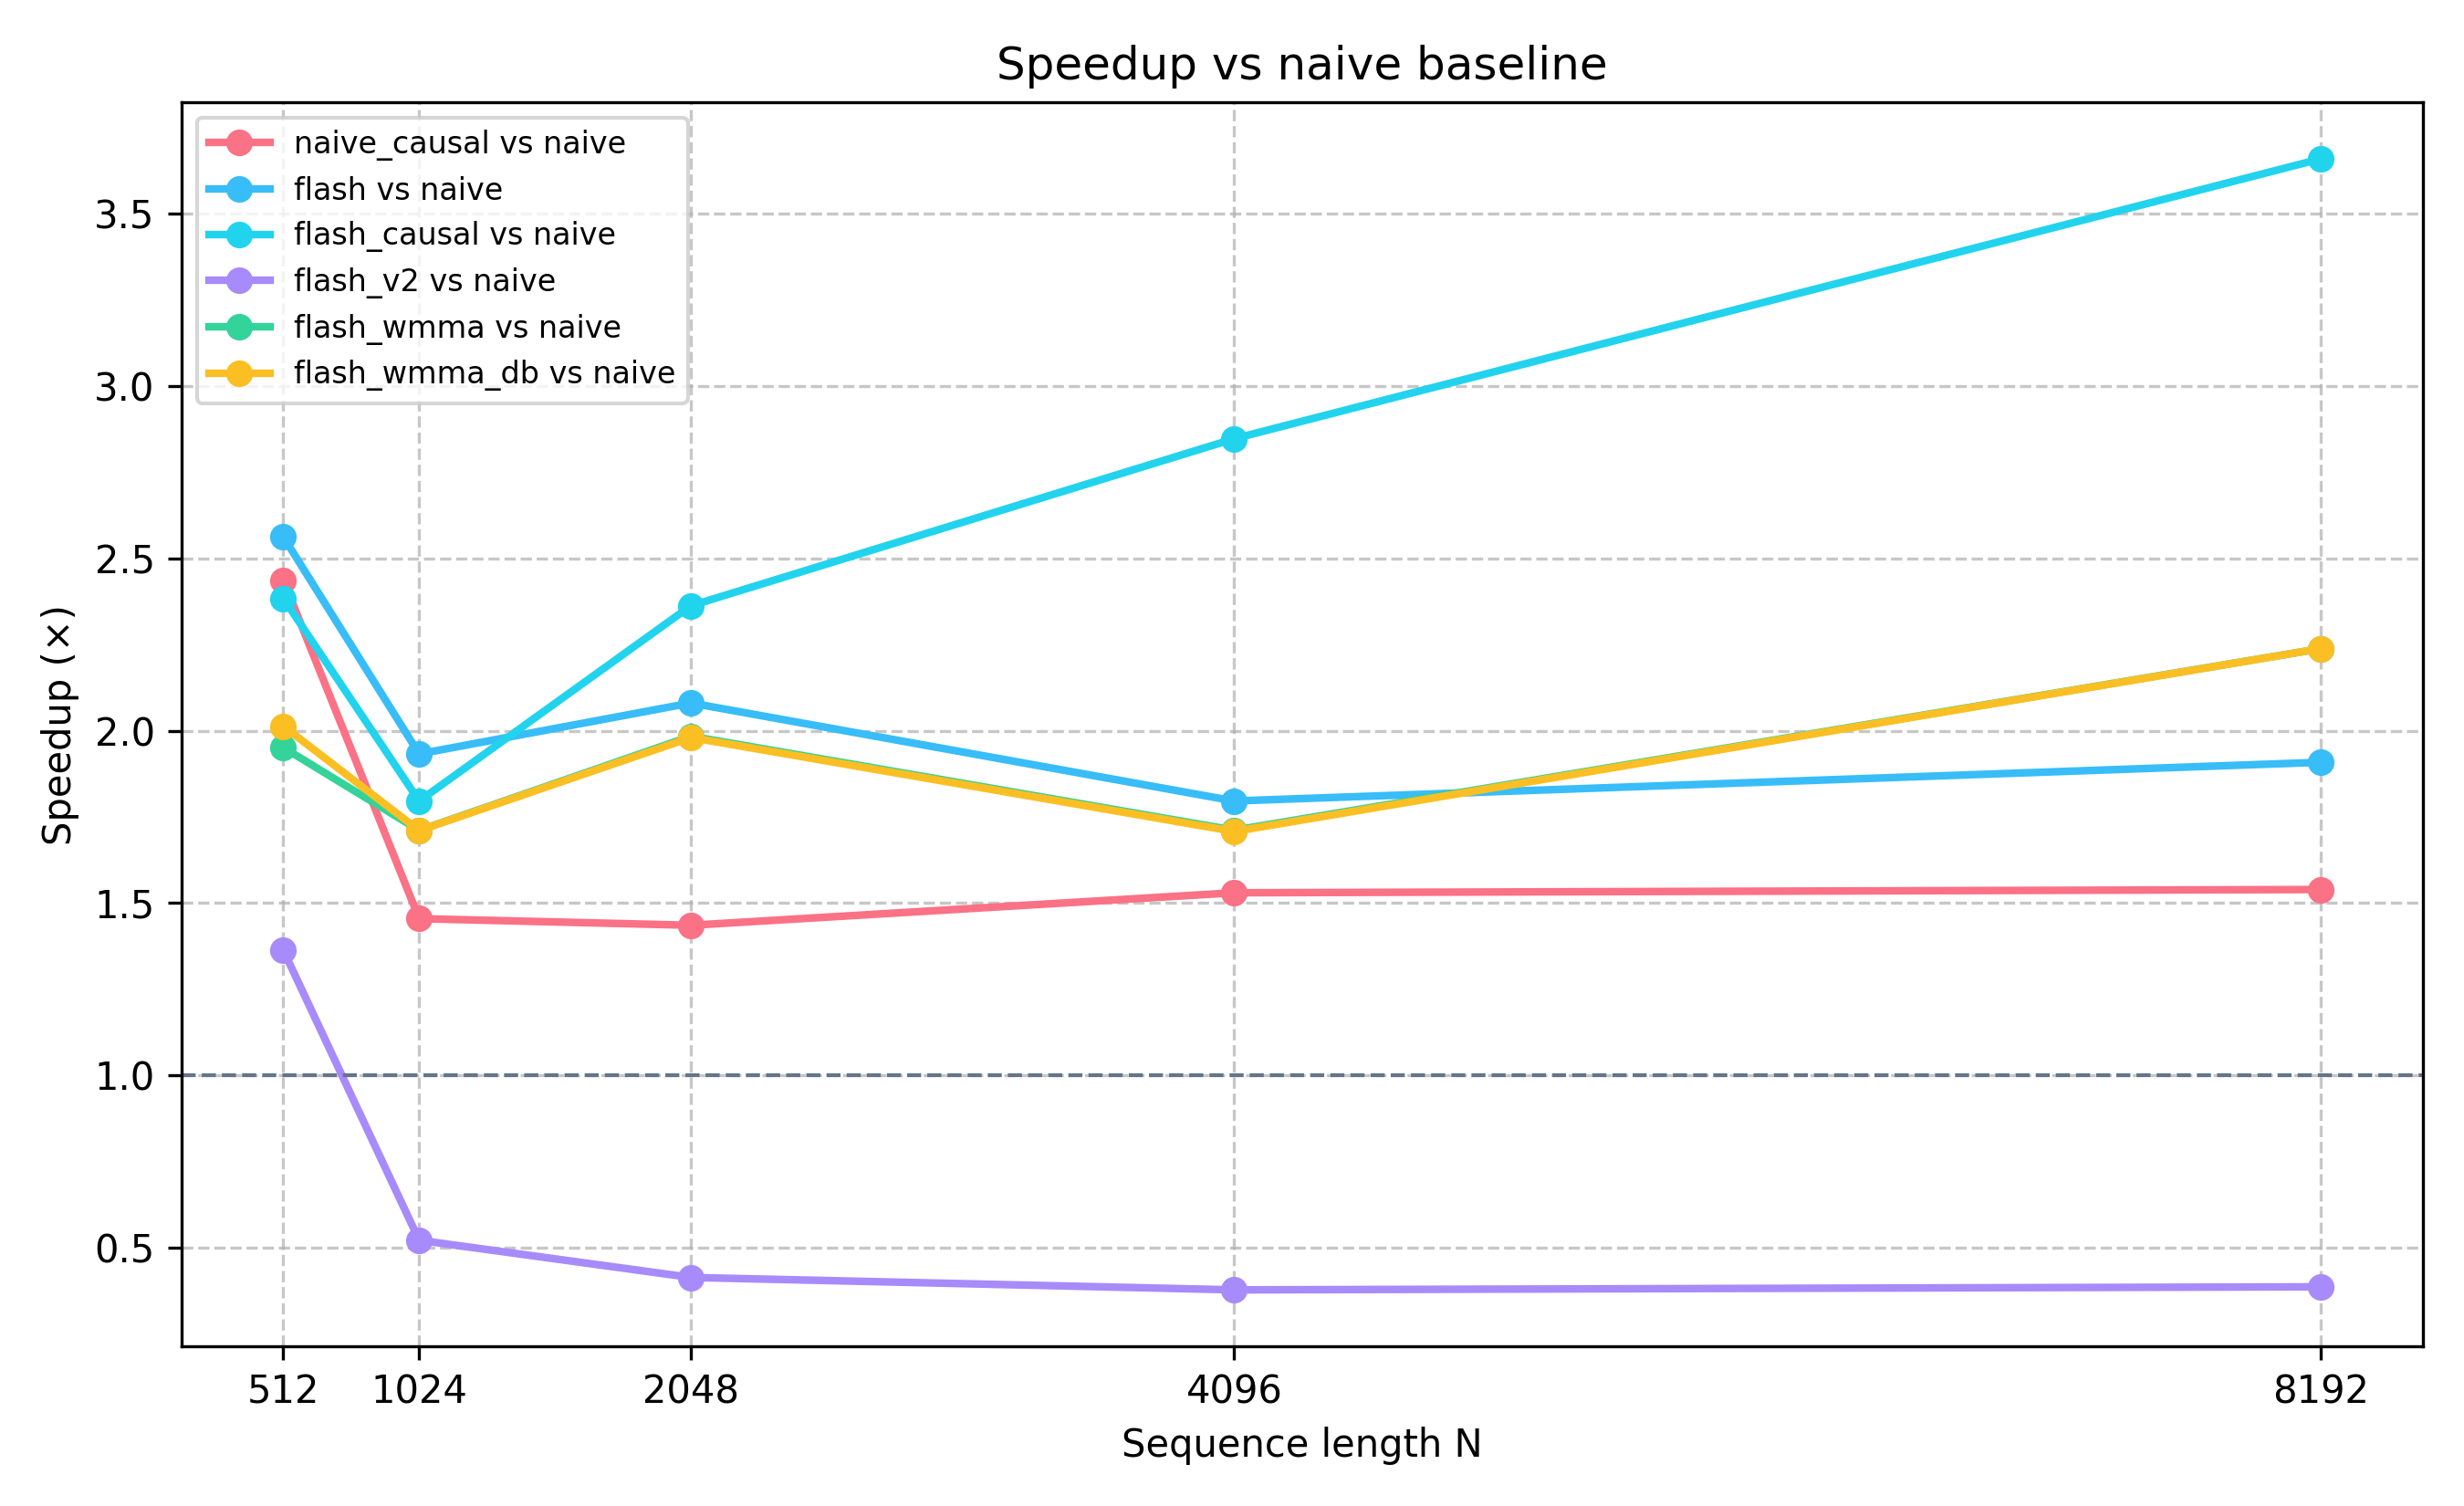
\includegraphics[width=0.75\textwidth]{docs/assets/speedup_plot.png}
    \caption{Speedup vs.\ \texttt{naive} across $N$.}
    \label{fig:speedup}
\end{figure}

\begin{table}[htbp]
    \centering
    \caption{Mean latency (ms), $d{=}64$, Tesla T4 (representative rows).}
    \label{tab:latency}
    \begin{tabular}{lrr}
        \toprule
        Kernel & $N{=}4096$ & $N{=}8192$ \\
        \midrule
        \texttt{naive} & 27.03 & 111.99 \\
        \texttt{naive\_causal} & 17.67 & 72.75 \\
        \texttt{flash} & 15.05 & 58.68 \\
        \texttt{flash\_causal} & 9.49 & 30.60 \\
        \texttt{flash\_v2} & 71.56 & 289.67 \\
        \texttt{flash\_wmma} & 15.79 & 50.03 \\
        \texttt{flash\_wmma\_db} & 15.83 & 50.03 \\
        \bottomrule
    \end{tabular}
\end{table}

\subsection{HBM Traffic Reduction}
Nsight Compute telemetry confirms the core hypothesis. For $N{=}4096$:
\begin{itemize}
    \item \textbf{Naive Traffic:} $\approx 25.2$\,GB read, $\approx 1.14$\,GB write (aggregated NCU metrics).
    \item \textbf{Flash Traffic:} $\approx 2.16$\,GB read, $\approx 8.2$\,MB write.
\end{itemize}
This represents an \textbf{$\approx 12\times$ reduction in reads} and an \textbf{$\approx 138\times$ reduction in writes} relative to naive at this sequence length.

\begin{figure}[htbp]
    \centering
    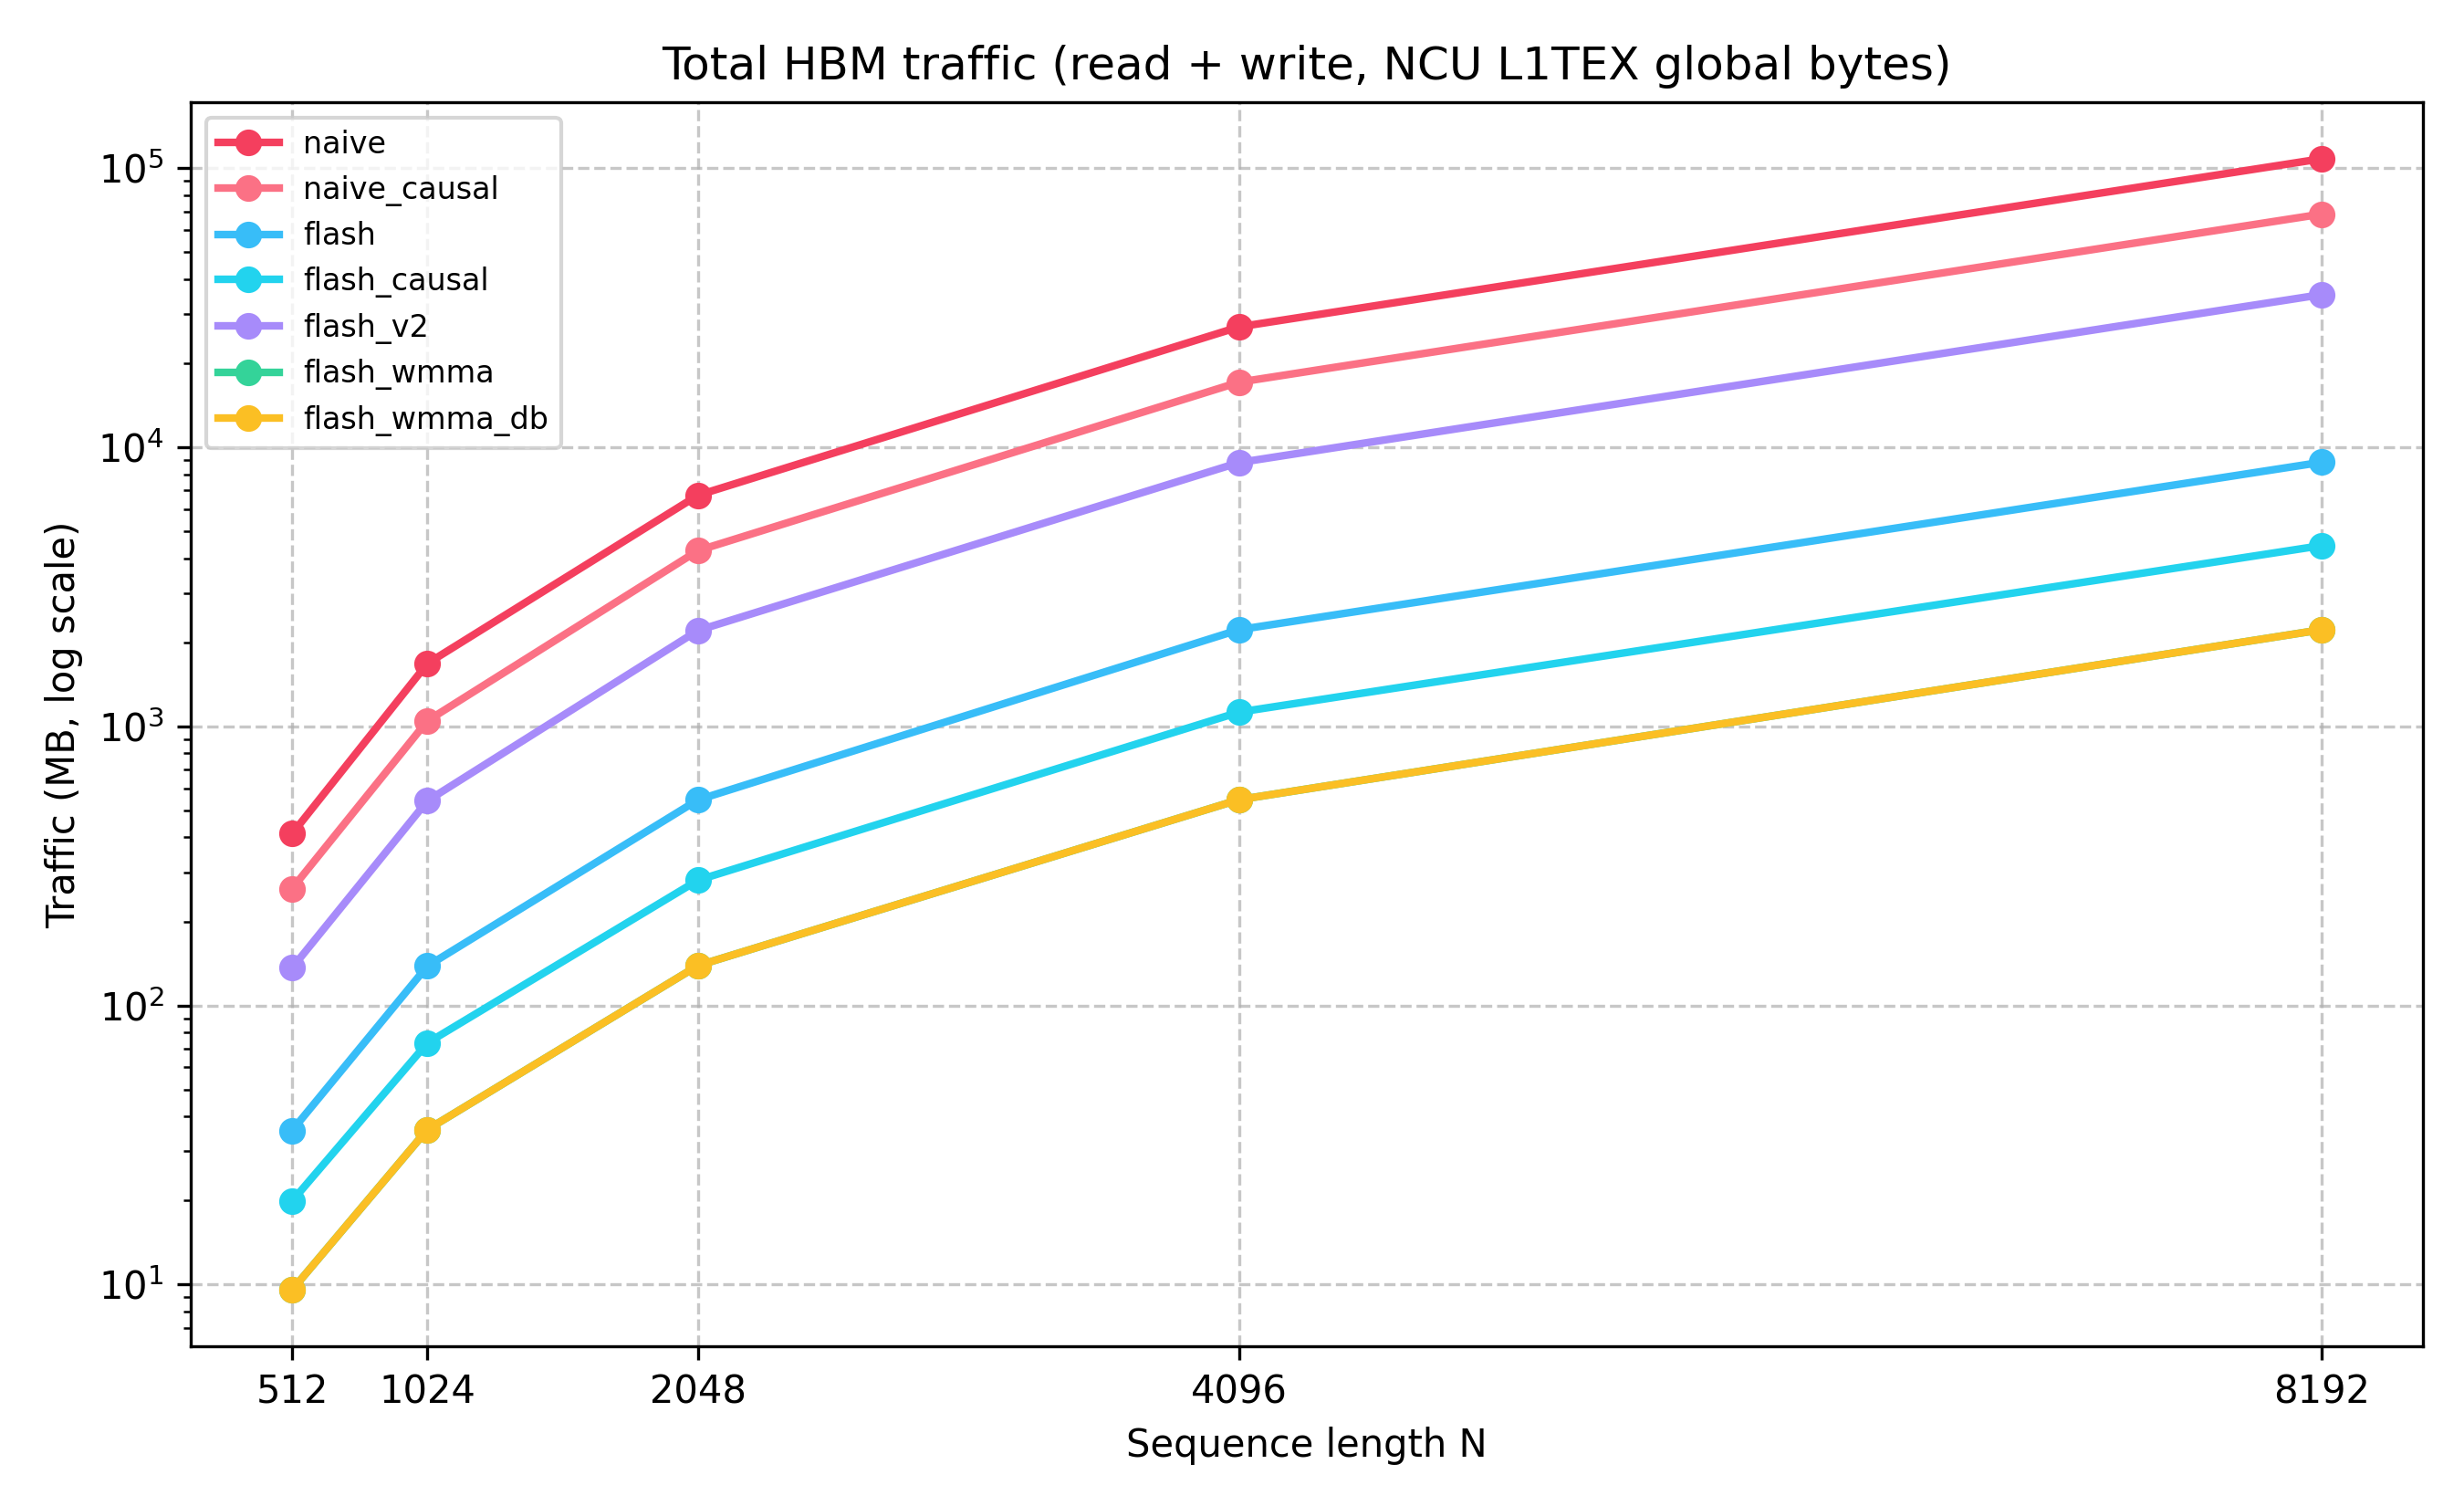
\includegraphics[width=0.75\textwidth]{docs/assets/hbm_plot.png}
    \caption{HBM Global Memory Traffic vs Sequence Length. Notice the quadratic scaling of the naive implementation.}
    \label{fig:hbm}
\end{figure}

\begin{table}[htbp]
    \centering
    \caption{NCU global loads + stores (MB), $N{=}8192$.}
    \label{tab:hbm8192}
    \begin{tabular}{lrrr}
        \toprule
        Kernel & Read & Write & Total \\
        \midrule
        \texttt{naive} & 103{,}352.3 & 4{,}663.5 & 108{,}015.8 \\
        \texttt{naive\_causal} & 63{,}785.0 & 4{,}663.7 & 68{,}448.7 \\
        \texttt{flash} & 8{,}816.6 & 16.8 & 8{,}833.4 \\
        \texttt{flash\_causal} & 4{,}423.7 & 16.8 & 4{,}440.5 \\
        \texttt{flash\_v2} & 35{,}194.9 & 16.8 & 35{,}211.7 \\
        \texttt{flash\_wmma} & 2{,}201.6 & 16.8 & 2{,}218.4 \\
        \texttt{flash\_wmma\_db} & 2{,}201.6 & 16.8 & 2{,}218.4 \\
        \bottomrule
    \end{tabular}
\end{table}

\subsection{Roofline-style Diagnostic}
Figure~\ref{fig:roofline} combines an analytical $4N^2d$ FLOP estimate with NCU byte totals (see \texttt{python/plot\_results.py}).

\begin{figure}[htbp]
    \centering
    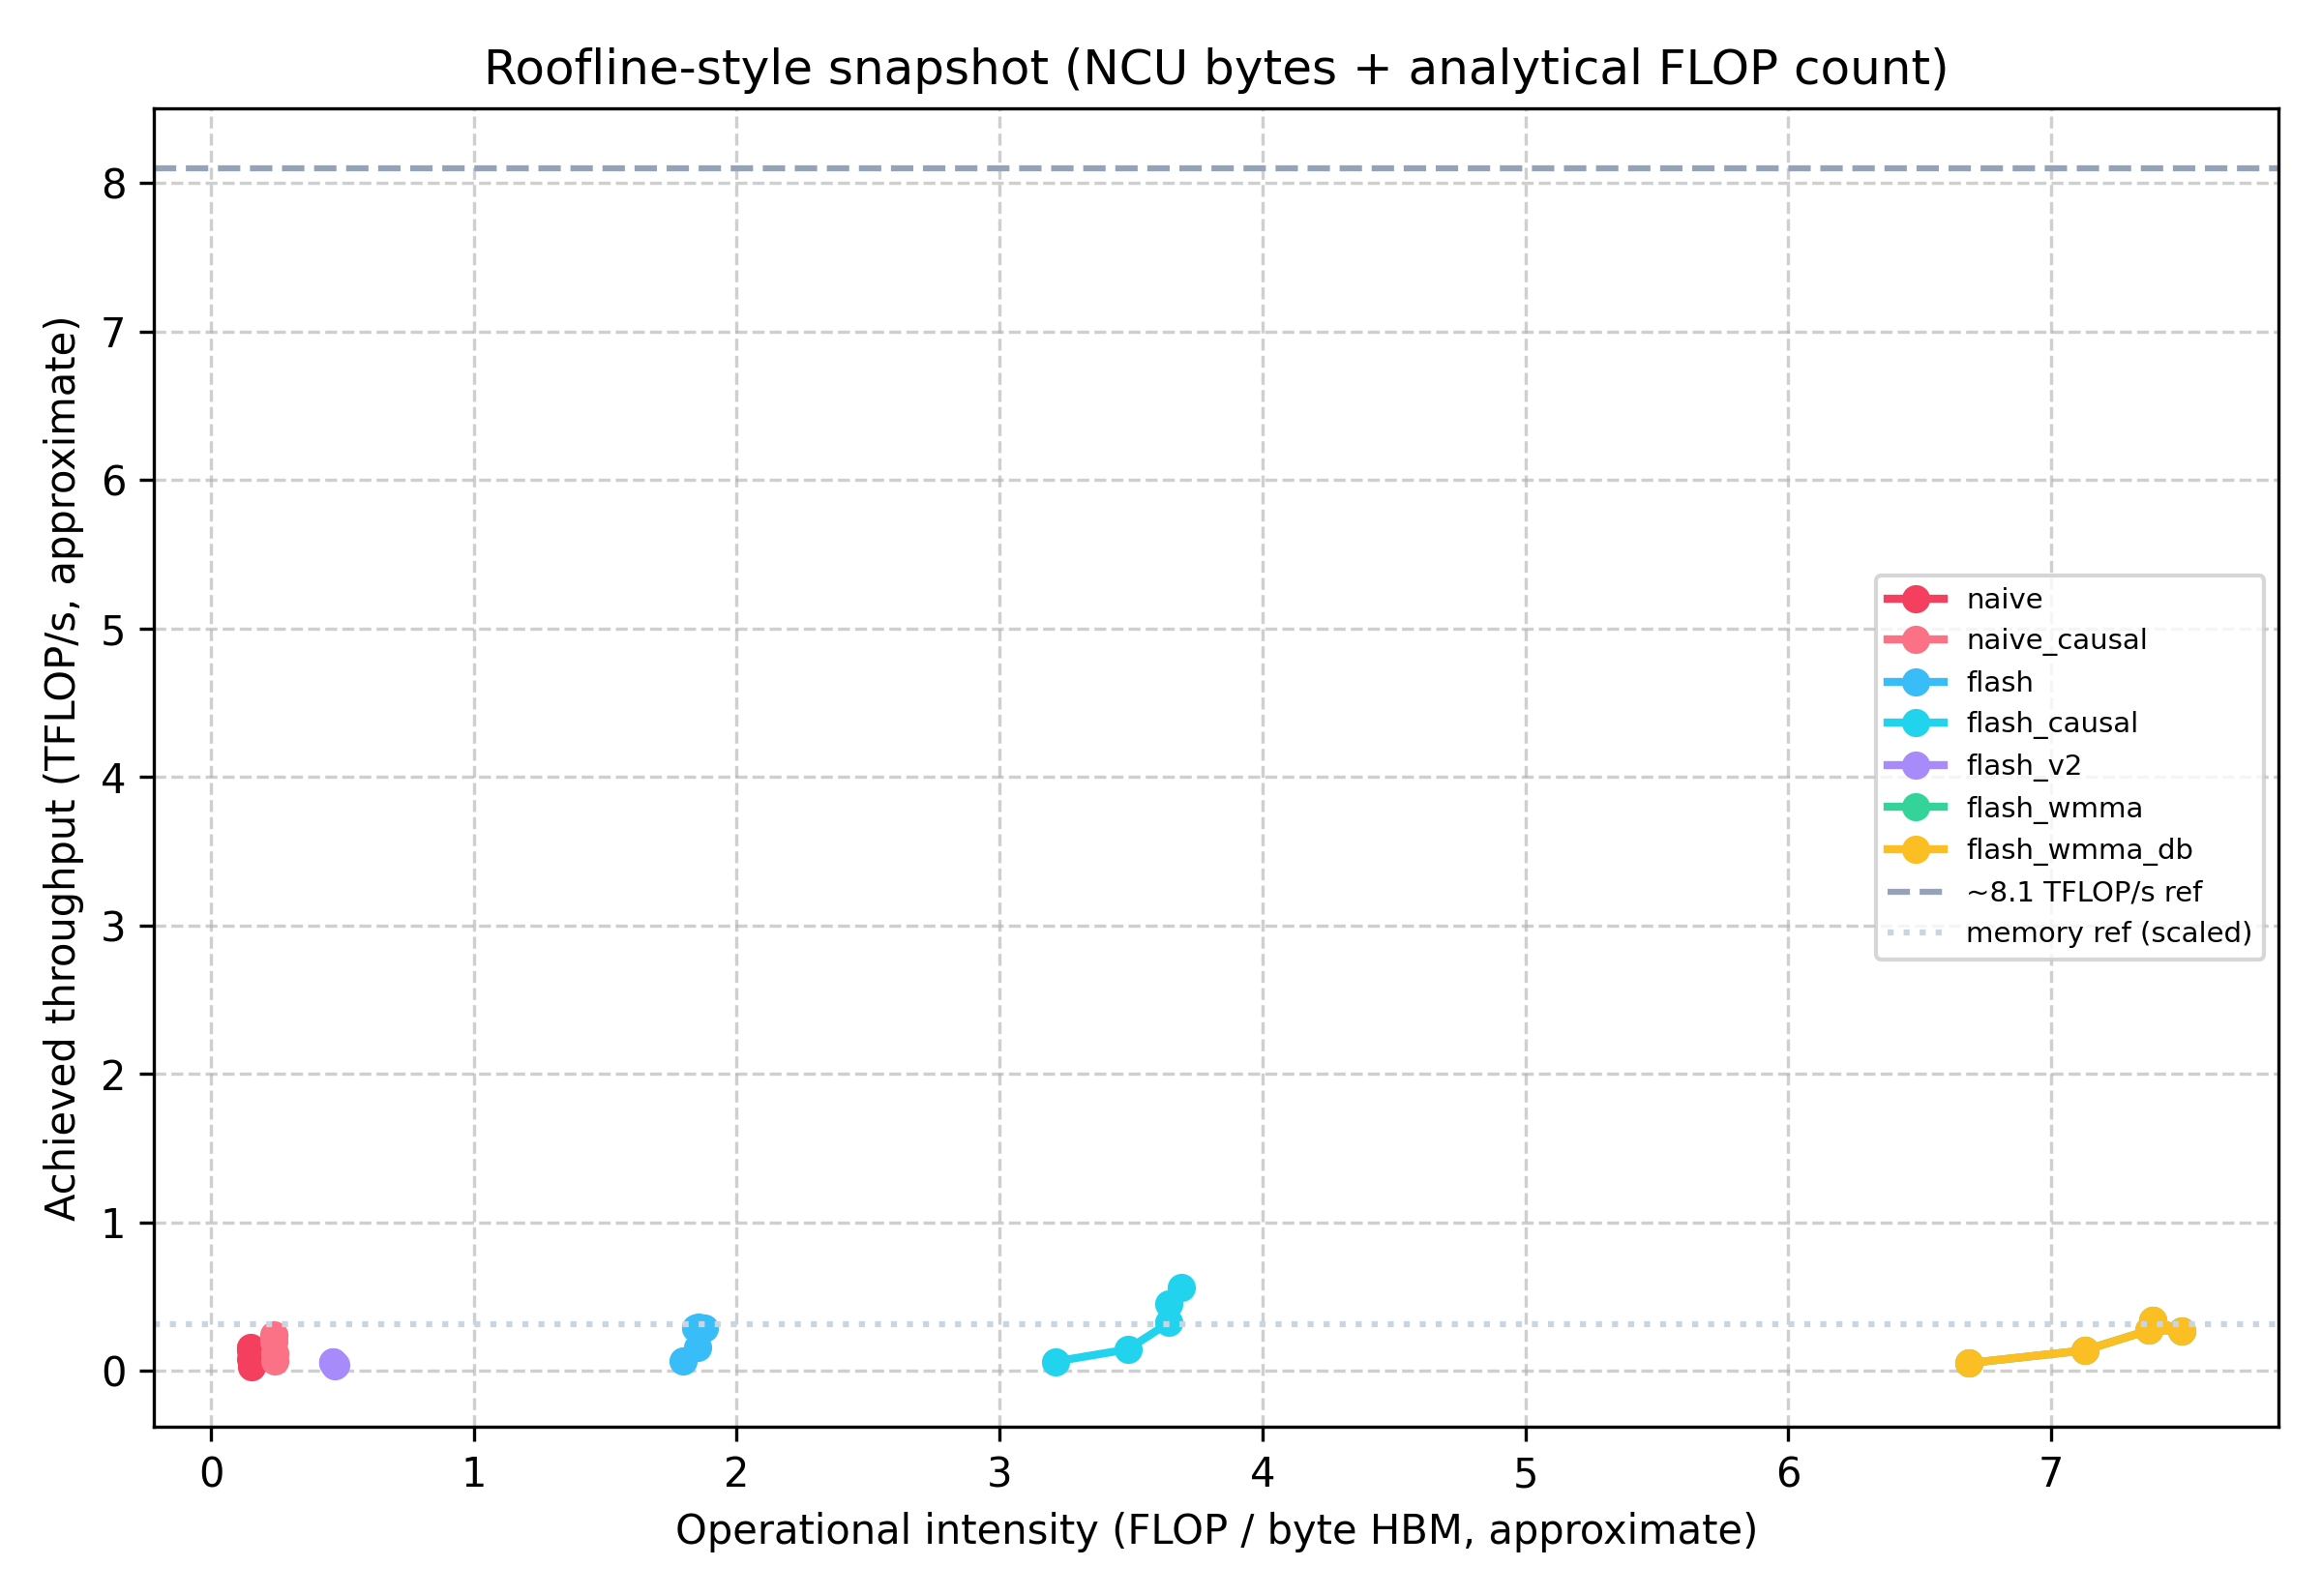
\includegraphics[width=0.72\textwidth]{docs/assets/roofline_plot.png}
    \caption{Roofline-style plot: approximate attained TFLOP/s vs operational intensity.}
    \label{fig:roofline}
\end{figure}

\subsection{Discussion}
\label{sec:discussion}
\begin{itemize}
    \item \textbf{Causal Flash} delivers the best wall-clock times here ($\approx 30.6$\,ms at $N{=}8192$), with NCU totals roughly half those of non-causal Flash for global reads.
    \item \textbf{WMMA} speeds up non-causal Flash ($\approx 50.0$\,ms) and shows the smallest read footprint in Table~\ref{tab:hbm8192}; it still trails causal Flash in latency unless causal masking and WMMA are fused (future work).
    \item \textbf{\texttt{flash\_wmma\_db}} matches WMMA on this GPU---no measured gain from the current double-buffer entry point on sm\_75.
    \item \textbf{\texttt{flash\_v2}} is slower than naive for large $N$ in this sweep and exhibits substantially higher NCU-reported reads than Flash v1; the warp-centric prototype requires redesign to be competitive.
\end{itemize}

\section{Interactive Educational Website}
Alongside the CUDA implementation, the project documentation has been transformed into a highly-readable technical blog hosted at \url{https://batra98.github.io/me759-flashattention}.

A dynamic, CSS-driven state machine visually simulates a single Streaming Multiprocessor, including a glowing Data Bus, Global Memory blocks, SRAM tiles, and a pulsing 32-thread Warp Grid. This provides users with a direct visual intuition of the $O(N^2)$ HBM bottleneck versus SRAM data locality.

\section{Future Work}
Remaining directions include fusing causal masking with WMMA tiles; revisiting warp-centric tiling with occupancy-aware configurations; KV-cache--aware inference kernels; and multi-GPU sequence-parallel attention (NCCL/MPI). FlashAttention-2/3 scheduling ideas remain relevant for further throughput~\cite{dao2022}.

\begin{thebibliography}{9}

\bibitem{dao2022}
Dao, T., Fu, D. Y., Ermon, S., Rudra, A., \& Ré, C. (2022).
\textit{FlashAttention: Fast and Memory-Efficient Exact Attention with IO-Awareness.}
NeurIPS 2022. \url{https://arxiv.org/abs/2205.14135}

\bibitem{vaswani2017}
Vaswani, A. et al. (2017).
\textit{Attention Is All You Need.}
NeurIPS 2017. \url{https://arxiv.org/abs/1706.03762}

\bibitem{milakov2018}
Milakov, M. \& Gimelshein, N. (2018).
\textit{Online normalizer calculation for softmax.}
arXiv preprint. \url{https://arxiv.org/abs/1805.02867}

\bibitem{nvidia_wmma}
NVIDIA.
\textit{CUDA C++ Programming Guide: Warp Matrix Functions (WMMA).}
\url{https://docs.nvidia.com/cuda/cuda-c-programming-guide/index.html#warp-matrix-functions}

\end{thebibliography}

\end{document}
